\documentclass[xcolor={usenames,dvipsnames}]{beamer}
\usetheme{CambridgeUS}
\usecolortheme{dolphin}
\usefonttheme{serif}

\setbeamercolor{block title alerted}{fg=black,bg=red}

\usepackage[english]{babel}
\usepackage[T1]{fontenc}
\usepackage[utf8]{inputenc}
\usepackage{bbold}
\usepackage{lmodern}
\newcommand{\argmin}{\arg\!\min}

\usepackage{multimedia}
\usepackage{tikz}
\usepackage{graphicx}
\usepackage{amsmath}
\usepackage{amsthm}
\usepackage{amsfonts}


\newtheorem{prop}{Proposition}
\newtheorem{rmk}{Remark}

%% %%%%%%%%%%%%%%%%%%%%%%%%%%%%%%%%%%%%%%%%%%%%%%%%%%%%%%%%%%%%%%%%%%%%%%%%%%%%%
%% %%%%%%% %% %% %  %                                      %  % %% %% %%%%%%%%%%
%%%%% %% %  %                    MES COMMANDES                     %  % %% %%%%%
%%%%%%%%%% %% %% %  %                                      %  % %% %% %%%%%%% %%
%%%%%%%%%%%%%%%%%%%%%%%%%%%%%%%%%%%%%%%%%%%%%%%%%%%%%%%%%%%%%%%%%%%%%%%%%%%%% %%


\newcommand{\zzpackages}[1][french]{
  \usepackage[utf8]{inputenc}
  \usepackage[T1]{fontenc}
  \usepackage[#1]{babel}

  \usepackage{amsthm}
  \usepackage{amsmath}
  \usepackage{amsfonts}
  \usepackage{amssymb}

  \usepackage{xcolor}
  \usepackage{xstring}	%\ifstreqcase
}

%% %%%%%%%%%%%%%%%%%%%%%%%%%%%%%%%%%%%%%%%%%%%%%%%%%%%%%%%%%%%%%%%%%%%%%%%%%%%%%
%                              TESTS / FOR / ...                               %
%%%%%%%%%%%%%%%%%%%%%%%%%%%%%%%%%%%%%%%%%%%%%%%%%%%%%%%%%%%%%%%%%%%%%%%%%%%%% %%

% 
\def\defactive#1#2{
  \catcode`#1=13
  \begingroup
  \lcode`~=`#1
  \lowercase{\endgroup\def~}{#2}
}

\def\zifempty#1#2#3{\def\foo{#1}\ifx\foo\empty\relax#2\else#3\fi}

%% %%%%%%%%%%%%%%%%%%%%%%%%%%%%%%%%%%%%%%%%%%%%%%%%%%%%%%%%%%%%%%%%%%%%%%%%%%%%%
%                           MARGES / HYPERREF / ...                            %
%%%%%%%%%%%%%%%%%%%%%%%%%%%%%%%%%%%%%%%%%%%%%%%%%%%%%%%%%%%%%%%%%%%%%%%%%%%%% %%

\makeatletter
\gdef\@subtitle{}
\def\subtitle#1{\gdef\@subtitle{#1}}

\def\zztitre{
\begingroup\centering
{\bfseries \huge \@title}\par\vspace{.3cm}
\ifx\@subtitle\empty\else{\bfseries \Large \@subtitle}\par\vspace{.5cm}\fi
\Large \@author\par\vspace{.1cm}
\@date\zal\vspace{.3cm}\zal
\zligne\endgroup
}

\makeatother


\newcommand{\zzhyperref}{
\usepackage{hyperref}
\hypersetup{ colorlinks=true, linkcolor=blue!30!black,
citecolor=green!30!black, filecolor=magenta!30!black,
urlcolor=cyan!30!black }
}

\newcommand{\zzmarges}{
  \setlength{\textheight}{620pt}
  \addtolength{\textwidth}{2cm}
  \addtolength{\hoffset}{-1cm}
  \addtolength{\voffset}{-1cm}
  \addtolength{\marginparwidth}{0cm}
  \addtolength{\textheight}{1cm}
} 

\makeatletter
\newcommand{\zzheader}[6]{
\def\@oddhead{\vbox to 0pt{\vss\hspace{0pt} #1\hfill #2\hfill #3\kern4pt\par\kern5pt\hrule height.5pt}}
\def\@oddfoot{\vbox to 0pt{\hrule height.5pt\kern5pt\hbox to \linewidth{\kern4pt {#4}\hss {#5}\hss {#6}\kern4pt}\vss}}}
\makeatother

%%%%%%%%%%%%%%%%%%%%%%%%%%%%%%%%%%%%%%%%%%%%%%%%%%%%%%%%%%%%%%%%%%%%%%%%%%%%%%%%

\newcommand{\zligne}[1][]{
\par\zifempty{#1}%
{\hbox to \linewidth{\leaders\hrule height3pt depth-2.5pt\hfill}}%
{\hbox to \linewidth{\leaders\hrule height3pt depth-2.5pt\hfill\kern.8em #1\kern.8em\leaders\hrule height3pt depth-2.5pt\hfill}}\par
}

%%%%%%%%%%%%%%%%%%%%%%%%%%%%%%%%%%%%%%%%%%%%%%%%%%%%%%%%%%%%%%%%%%%%%%%%%%%%%%%%

\newcommand{\zal}{\par}
\newcommand{\znl}{\zal ~\zal}
\newcommand{\zguill}[2][]{«\,#2\,»}

%% %%%%%%%%%%%%%%%%%%%%%%%%%%%%%%%%%%%%%%%%%%%%%%%%%%%%%%%%%%%%%%%%%%%%%%%%%%%%%
%                             COMMANDES PRATIQUES                              %
%%%%%%%%%%%%%%%%%%%%%%%%%%%%%%%%%%%%%%%%%%%%%%%%%%%%%%%%%%%%%%%%%%%%%%%%%%%%% %%

%% ------- -- -- -  -                                      -  - -- -- --------%%
%---- -- -  -                          ZP                          -  - -- ----%
%%-------- -- -- -  -                                      -  - -- -- ------- %%
\makeatletter
\def\z@first#1#2{#1}
\def\z@second#1#2{#2}
\def\z@zp@selectchar#1#2{
  \IfStrEqCase{#2}{%
    {p}{#1{(}{)}}%
    {c}{#1{[}{]}}%
    {a}{#1{\{}{\}}}%
    {C}{#1{]}{[}}%
    {b}{#1{|}{|}}%
    {n}{#1{\|}{\|}}%
    {i}{#1{[}{]}\!#1{[}{]}}%
    {t}{#1{<}{>}}%
    {v}{#1{.}{.}}%
    {A}{#1{\}}{\{}}%
    {P}{#1{)}{(}}%
    {I}{#1{]}{[}\!#1{]}{[}}%
    {T}{#1{>}{<}}%
  }[#1{(}{)}]%
}

\def\z@zp#1#2\fin#3{
  \z@zp@selectchar{\left\z@first}{#1}#3
  \zifempty{#2}%
        {\z@zp@selectchar{\right\z@second}{#1}}%
        {\z@zp@selectchar{\right\z@second}{#2}}%
}
\newcommand{\zp}[2][]{\zifempty{#1}{\left(#2\right)}{\z@zp#1\fin{#2}}}

\newcommand{\zpbig}[1]{\ifcase#1\relax\vrule width0pt height0pt\or\vrule width0pt height9pt\or\vrule width0pt height10pt\or\vrule width0pt height13pt\else\vrule width0pt height16pt\fi}

%% ------- -- -- -  -                                      -  - -- -- --------%%
%---- -- -  -                   Itemize et autre                   -  - -- ----%
%%-------- -- -- -  -                                      -  - -- -- ------- %%

\newcommand{\zitemize}[1]{
\vspace{-\topsep}\begin{itemize}\setlength\itemsep{0pt plus 1pt}\setlength\parskip{0cm}#1\end{itemize}\vspace{-\topsep}}


%% ------- -- -- -  -                                      -  - -- -- --------%%
%---- -- -  -                        AUTRES                        -  - -- ----%
%%-------- -- -- -  -                                      -  - -- -- ------- %%

\newcommand{\zR}{\mathbb{R}}

\newcommand{\zsum}[2][0pt]{\sum_{\hbox to #1{\hss$\scriptstyle#2$\hss}}}
\newcommand{\zprod}[2][0pt]{\prod_{\hbox to #1{\hss$\scriptstyle#2$\hss}}}

\newcommand{\zseq}[1][=]{\hspace{2pt}\raise .5pt\hbox{\scalebox{.8}{#1}}\hspace{2pt}}

\newcommand{\zop}[2]{\mathrm{#1}\zp{#2}}

\newcommand{\zi}{\mathrm{i}}

\newcommand{\zexp}[1]{\mathrm{e}^{#1}}

\newcommand{\zmatrix}[2]{\left(\begin{array}{#1}#2\end{array}\right)}

\newcommand{\zindic}[1]{%
\hbox to 5.3pt{1\hss l}\hskip -2.5pt\left\{#1\right\}%
}

\newcommand{\zesp}[2][]{%              esperance
\mathbb{E}_{#1}\hskip -3pt\left[\zpbig1\,#2\,\right]%
}

\newcommand{\zprob}[2][]{%             proba
\mathbb{P}_{#1}\hskip -3pt\left(\zpbig1\,#2\,\right)%
}

% Symbole d'indépendance de variable aléatoire
\newcommand{\zindep}{\protect\mathpalette{\protect\z@ind}{\perp}}
\def\z@ind#1#2{\mathrel{\rlap{$#1#2$}\mkern6mu{#1#2}}}


\newcommand{\zdx}[1]{\mathrm{d}#1}

\newcommand{\zderiv}[2]{\frac{\partial #1}{\partial #2}}


\newcommand{\ztr}[2][]{\zifempty{#1}{#2}{\left(#2\right)}^{\hspace{-1pt}\mathsf{T}}\hspace{-1pt}}
\def\zpreind#1#2{ \raise-.35ex\hbox{\scriptsize$#1$}#2}
\def\zpreexp#1#2{ \raise.85ex\hbox{\scriptsize$#1$}#2}

%% %%%%%%%%%%%%%%%%%%%%%%%%%%%%%%%%%%%%%%%%%%%%%%%%%%%%%%%%%%%%%%%%%%%%%%%%%%%%%
%                                 ALGORITHMES                                  %
%%%%%%%%%%%%%%%%%%%%%%%%%%%%%%%%%%%%%%%%%%%%%%%%%%%%%%%%%%%%%%%%%%%%%%%%%%%%% %%

\newcount\z@algo@count
\newdimen\z@algo@indent
\begingroup
  \catcode`\^^M=13             %
  \catcode`\^^I=13             %
  \gdef\z@algo{                %
  \z@algo@count=1
    \begingroup                %
    \catcode`\^^M=13           %
    \def^^M{\leavevmode\par \advance\z@algo@count by 1\z@algo@indent=0pt}%
    \catcode`\^^I=13           %
    \def^^I{\advance\z@algo@indent by 1em}         %
    \everypar{                 %
      \hbox to 0cm{\hss\textcolor{black!30}{\the\z@algo@count~:}}~\kern\z@algo@indent}  %
                               %
    \tt                        %
  }

\endgroup

\newenvironment{zalgo}{\z@algo}{\endgroup}


\makeatother



%% %%%%%%%%%%%%%%%%%%%%%%%%%%%%%%%%%%%%%%%%%%%%%%%%%%%%%%%%%%%%%%%%%%%%%%%%%%%%%
%                                    AUTRE                                     %
%%%%%%%%%%%%%%%%%%%%%%%%%%%%%%%%%%%%%%%%%%%%%%%%%%%%%%%%%%%%%%%%%%%%%%%%%%%%% %%

% epaisseur trait / marge / texte

\def\zfbox#1#2#3{
  \hbox{\vrule width #1
    \vtop{
      \vbox{
        \hrule height #1
        \kern #2
        \hbox{\kern #2 #3\kern #2}
      }%
      \kern #2%
      \hrule height #1
    }%
    \vrule width #1%
  }%
}

%% \begin{mygraph}{xmin=0, xmax=1, %
%%                ymin=0, ymax=1, %
%%                sizex=2.5, sizey=2.5}%
%%                {nomx=Axe X, nomy=Axe Y}%
%%                {0,.5,1}{0,0.25,...,1.05}

%% \graduationX[dashed, blue]{ .78 / $\frac{\pi}{4}$ }{ PARAMETRE TEXT }

%% \begin{mylegend}{x=0.3, y=.9, n=2, t=2.1, scale=.5}
%%   \newlegend{blue}{Courbe 1}
%%   \newlegend{red}{Courbe 2}
%% \end{mylegend}

%% \fillbetweencurve[opacity=.2, blue]{ COURBE 1 }{ COURBE 2 }

%% \end{mygraph}


\usepackage{tikz}



\pgfkeys{
%
 /mygraph/.is family, /mygraph,
 xmin/.estore in = \xn,
 xmax/.estore in = \xm,
 ymin/.estore in = \yn,
 ymax/.estore in = \ym,
 sizex/.estore in = \xx,
 sizey/.estore in = \yy,
 %
/mygraphb/.is family, /mygraphb,
 nomx/.estore in = \axex,
 nomy/.estore in = \axey,
%
/mygraphc/.is family, /mygraphc,
 gradsize/.estore in = \gradsize,
 gradsize/.default = 0.1,
 nomydist/.estore in = \axeyd,
 nomydist/.default = 0.8cm,
 gradsize, nomydist,                 % NE PAS OUBLIER
%
/myleg/.is family, /myleg,
 x/.estore in = \legendx,
 y/.estore in = \legendy,
 n/.estore in = \legendn,
 t/.estore in = \legendt,
 scale/.estore in = \legends,
 scale/.default = 1,
 scale,
%
/mylego/.is family, /mylego,
size/.estore in = \legendwidth,
size/.default = 0.4,
size                                  % NE PAS OUBLIER
}


%%%%%%%%%%%%%%%%%%%%%%%%%%%%%%%%%%%%%%%%%%%%%%%%%%%%%%%%%%%%%%%%%%%%%%%%%%%%%%%%
%                                                                              %
%%%%%%%%%%%%%%%%%%%%%%%%%%%%%%%%%%%%%%%%%%%%%%%%%%%%%%%%%%%%%%%%%%%%%%%%%%%%%%%%

\newenvironment{mygraph}[5][]{%
\pgfkeys{/mygraph, #2}
\pgfkeys{/mygraphb, #3}
\pgfkeys{/mygraphc, #1}
  \pgfmathsetmacro\dum{\yy/(\ym-\yn)}
  \pgfmathsetmacro\dumm{\xx/(\xm-\xn)}
\begin{tikzpicture}[yscale=\dum, xscale=\dumm,font=\sffamily]
  \pgfmathsetmacro\gradx{\gradsize / \dum}
  \pgfmathsetmacro\grady{\gradsize / \dumm}

  \foreach \x in {#4}{
    \draw[very thin, color=black, dotted] (\x,\yn) -- (\x,\ym);
    \draw (\x,\yn+\gradx) -- (\x,\yn)
          node[font=\tiny, anchor=north] {\pgfmathprintnumber{\x}};
  };
  \foreach \y in {#5}{
    \draw[very thin, color=black, dotted] (\xn,\y) -- (\xm,\y); 
    \draw (\xn+\grady,\y) -- (\xn,\y)
          node[font=\tiny, anchor=east] {\pgfmathprintnumber{\y}};
  };
  \draw (\xn,\yn) -- node[font=\scriptsize, below=0.3cm] {\axex} (\xm,\yn);
  \draw (\xn,\yn) -- node[font=\scriptsize, rotate=90, above=\axeyd, anchor=mid] {\axey} (\xn,\ym);
  \draw (\xn,\ym) -- (\xm,\ym);
  \draw (\xm,\yn) -- (\xm,\ym);

  \begin{scope}
    \clip (\xn,\yn) rectangle (\xm,\ym);
    %% \draw[dashed] (\xn, 0) -- (\xm, 0);
    %% \draw[dashed] (0, \yn) -- (0, \ym);
}{
  \end{scope}
\end{tikzpicture}
}

%%%%%%%%%%%%%%%%%%%%%%%%%%%%%%%%%%%%%%%%%%%%%%%%%%%%%%%%%%%%%%%%%%%%%%%%%%%%%%%%

\newenvironment{mylegend}[2][]{
\pgfkeys{/myleg, #2}
\pgfkeys{/mylego, #1}
\begin{scope}[shift={(\legendx,\legendy)}, scale=\legends]
\pgfmathsetmacro\legendwidth{\legendwidth * (\xm-\xn) / \xx }
\pgfmathsetmacro\dum{ (0.125 * (\ym-\yn) / \yy) }
\pgfmathsetmacro\dumm{ - (0.125 * (\xm-\xn) / \xx) }
\pgfmathsetmacro\legendy{ 0 }
\coordinate (dum) at (\dumm,\dum);
\pgfmathsetmacro\dum{ - (\legendn-0.4)*(0.25 * (\ym-\yn) / \yy) }
\coordinate (dumm) at (\dumm,\dum);
\pgfmathsetmacro\dumm{\dumm + (\legendt * (\xm-\xn) / \xx) }
\draw[fill=white, opacity=.8] (dum) -- (dumm) -| (\dumm,\dum) |- (dum);
}{
\end{scope}
%% \pgfmathsetmacro\legendyi{\legendyi + (0.125 * (\ym-\yn) / \yy)  }
%% \pgfmathsetmacro\legendy{\legendy + (0.1 * (\ym-\yn) / \yy)  }
%% \pgfmathsetmacro\legendx{\legendx - (0.125 * (\xm-\xn) / \xx)  }
%% \draw[] (\legendx,\legendyi) -- (\legendx,\legendy) %
%%                              -| (\legendx + 1,\legendy)
%%                              |- (\legendx,\legendyi);
}

\newcommand{\newlegend}[2]{
\draw[font=\scriptsize, #1] (0,\legendy) -- (\legendwidth,\legendy)	node[right,scale=\legends]{#2};
\pgfmathsetmacro\legendy{\legendy - (0.25 * (\ym-\yn) / \yy)  }
}

%%%%%%%%%%%%%%%%%%%%%%%%%%%%%%%%%%%%%%%%%%%%%%%%%%%%%%%%%%%%%%%%%%%%%%%%%%%%%%%%

\newenvironment{outofbox}{%
  \end{scope}%
}{%
  \begin{scope}%
    \clip (\xn,\yn) rectangle (\xm,\ym);%
}

%%%%%%%%%%%%%%%%%%%%%%%%%%%%%%%%%%%%%%%%%%%%%%%%%%%%%%%%%%%%%%%%%%%%%%%%%%%%%%%%

\newcommand{\fillbetweencurve}[3][]{
\begin{scope}
\clip (\xn,\yn) -- #2 -- (\xm,\yn) -- cycle;
\fill[#1] (\xn,\ym) -- #3 -- (\xm,\ym) -- cycle;
\end{scope}
}

%%%%%%%%%%%%%%%%%%%%%%%%%%%%%%%%%%%%%%%%%%%%%%%%%%%%%%%%%%%%%%%%%%%%%%%%%%%%%%%%

\newcommand{\graduationX}[3][very thin, color=black, dotted]{
\end{scope}
  \foreach \x/\t in {#2}{
    \draw[#1] (\x,\yn) -- (\x,\ym);
    \draw (\x,\yn+\gradx) -- (\x,\yn)
          node[font=\tiny, anchor=north, #3] {\t};
  };
\begin{scope}%
\clip (\xn,\yn) rectangle (\xm,\ym);%
}

%%%%%%%%%%%%%%%%%%%%%%%%%%%%%%%%%%%%%%%%%%%%%%%%%%%%%%%%%%%%%%%%%%%%%%%%%%%%%%%%

\newcommand{\graduationY}[3][very thin, color=black, dotted]{
\end{scope}
  \foreach \y/\t in {#2}{
    \draw[#1] (\xn,\y) -- (\xm,\y);
    \draw (\xn+\grady,\y) -- (\xn,\y)
          node[anchor=east, font=\tiny, shift={(-0*\grady,0)}, #3] {\t};
  };
\begin{scope}%
\clip (\xn,\yn) rectangle (\xm,\ym);%
}

\tikzset{
zplot/.style={opacity=.8}
}
\hypersetup{ colorlinks=true, linkcolor=blue,
	citecolor=green, filecolor=magenta,
	urlcolor=cyan }

\begin{document}

\AtBeginSection[]
{
  \begin{frame}
  \frametitle{Contents}
  {\tableofcontents[currentsection, hideallsubsections]}
  \end{frame}
}

\title{MVA Reinforcement Learning}
\subtitle{Optimization of very difficult functions}
\author{Nathan de Lara, Florian Tilquin}
\date{January 25 2016}


\begin{frame}
\titlepage
\end{frame}

\usebackgroundtemplate{ }

\section*{Plan}
%\begin{frame}
%  \tableofcontents[]
%\end{frame}

\section{Introduction}
\begin{frame}
\frametitle{Problem Statement}
Given a function $f$, the goal is:
\begin{equation}
\mbox{maximize } f(x) \mbox{ for } x\in [0,1]^p
\end{equation}
Assumptions: $f$ is potentially:
\begin{itemize}
\item complicated to evaluate
\item not smooth
\item noisy
\end{itemize}
\end{frame}

\begin{frame}
\frametitle{The Multi-Armed Bandit}
Idea:
\begin{itemize}
\item Set a tree structure $\mathcal{T}$ over $[0,1]^p$, such that for each depth $h$, the set of nodes is a partition of the space
\item Define a sequence $(x_t,y_t)=(\mathcal{U}(I_{h_t,i_t}),f(x_t)+\xi_t)$
\item Choose $h_{t+1},i_{t+1}$ in function of $(x_{t'},y_{t'})_{t'<t}$
\end{itemize}
The construction can be set to minimize either:
\begin{itemize}
\item Simple regret: \begin{equation}
\underset{t\le T_{max}}{argmin}|f^*-y_t|
\end{equation}
\item Cumulative regret: \begin{equation}\underset{t\le T_{max}}{\sum}|f^*-y_t| \end{equation}
\end{itemize}
\end{frame}

\section{Algorithms}
\begin{frame}
\frametitle{HOO and POO}
This algorithm is called \textit{Optimistic} because its idea is to sequentially building a tree and try the most promising children.\\
\textbf{Upper bound:} $B_{h,i}=min(U_{h,i},max(B_{h+1,2i-1},B_{h,2i}))$ where:
\begin{equation}
\label{uhoo}
U_{h,i}=\widehat{\mu}_{h,i}+\nu \rho^h+\sqrt{\dfrac{2\log(T_{max})}{n_{h,i}}}
\end{equation}
\textbf{Update rule:} At each time step, the most promising child with respect to B is added to the tree.
\end{frame}

\begin{frame}
\frametitle{HCT}
In order to be pulled, an arm must maximize $B$ among the arms that have not been pulled enough yet. In order to reduce computational cost, $U$ is refreshed only when $t$ is a power of 2.\\
\textbf{Upper bound:} $B_{h,i}=min(U_{h,i},max(B_{h+1,2i-1},B_{h,2i}))$ where:
\begin{equation}
\label{uhct}
U_{h,i}=\widehat{\mu}_{h,i}+\nu \rho^h+\sqrt{\dfrac{c^2\log(1/min(1,\frac{c_1\delta}{2^{\lfloor \log(t) \rfloor + 1}}))}{n_{h,i}}}
\end{equation}
\textbf{Update rule:} Only the leaves of the current covering tree that have not been pulled enough with respect to a certain threshold $\tau_h(t)$ are expanded.
\end{frame}

\begin{frame}
\frametitle{StoSOO}
This algorithm is called \textit{simultaneous} because it can perform at each time steps as many evaluations as the depth of its current covering tree. Each node a its own evaluation budget $k$ in order no to spend to much budget on the first nodes.\\
\textbf{Upper bound:} In order to be pulled, a leaf must both have a positive remaining individual budget and maximize $B$ among the leaves of the same depth:
\begin{equation}
\label{bsoo}
B_{h,i}=\widehat{\mu}_{h,i}+\sqrt{\dfrac{\log(\frac{T_{max}k}{\delta})}{2n_{h,i}}}
\end{equation}
\textbf{Update rule:} Once a node that maximizes $B$ has used its entire budget, it is expanded.
\end{frame}

\begin{frame}
\frametitle{ATB}
The tree is not sequentially built but given as an input and the evaluations are performed among a set of \textit{active boxes} or \textit{active nodes}. The statistics of the children of active nodes are updated each time an arm is pulled.\\
\textbf{Upper bound:} At each time step, the arm pulled is chosen among the active nodes and maximizes:
\begin{equation}
B_{h,i} = \widehat{\mu}_{h,i}+(1+2\nu)r_{h,i}
\end{equation}
where $r_{h,i}=2\sqrt{\dfrac{\log[2^{h+1}(\tau+n_{h,i})]}{n_{h,i}}}$ is the confidence radius of the interval.\\
\textbf{Update rule:} If an active node has a radius small enough compared to the ones of its children, it is removed and replaced by them.
\end{frame}

\section{Results}
\begin{frame}
\frametitle{Tested functions}
\begin{figure}
\label{fig:functions}
\hbox{\hspace{-1.0cm}\begin{mygraph}{xmin=0, xmax=1, %
                ymin=0, ymax=1, %
                sizex=3, sizey=3}%
                {nomx=zbra, nomy=zbra}%
                {0,0.25,...,1}{0,0.25,...,1}
  \draw[zplot, blue] plot file {Data/Prodsin.data};
\end{mygraph}\hspace{-1cm}
\begin{mygraph}{xmin=0, xmax=1, %
                ymin=0, ymax=1, %
                sizex=3, sizey=3}%
                {nomx=zbra, nomy=zbra}%
                {0,0.25,...,1}{0,0.25,...,1}
  \draw[zplot, blue] plot file {Data/Garland.data};
\end{mygraph}\hspace{-1cm}
\begin{mygraph}{xmin=0, xmax=1, %
                ymin=-0.75, ymax=0.25, %
                sizex=3, sizey=3}%
                {nomx=zbra, nomy=zbra}%
                {0,0.25,...,1}{-0.75,-0.5,...,0.25}
  \draw[zplot, blue] plot file {Data/Grill.data};
\end{mygraph}\hss}
\caption{From the left to the right: Two-sine product, Garlang, Grill.}
\end{figure}
\end{frame}

\begin{frame}
\frametitle{Experimental protocol}
For $T_{max}=1000,5000$ we record:
\begin{itemize}
	\item The abscissa $x \in X$ the algorithm went through
	\item The reward $rew(x)$ it obtained
\end{itemize}
And compare the algorithms over:
\begin{itemize}
	\item Cumulative regret $\tilde{R}$
	\item Simple regret $R$
	\item Best result
	\item Computation time
\end{itemize}

\end{frame}

\begin{frame}
\frametitle{Sampled points}
%%%%%%%%%%%%%%%%%%%%%%%%%%%  POSITIONS 1000 POINTS  %%%%%%%%%%%%%%%%%%%%%
\begin{figure}
\vspace{-0.5cm}
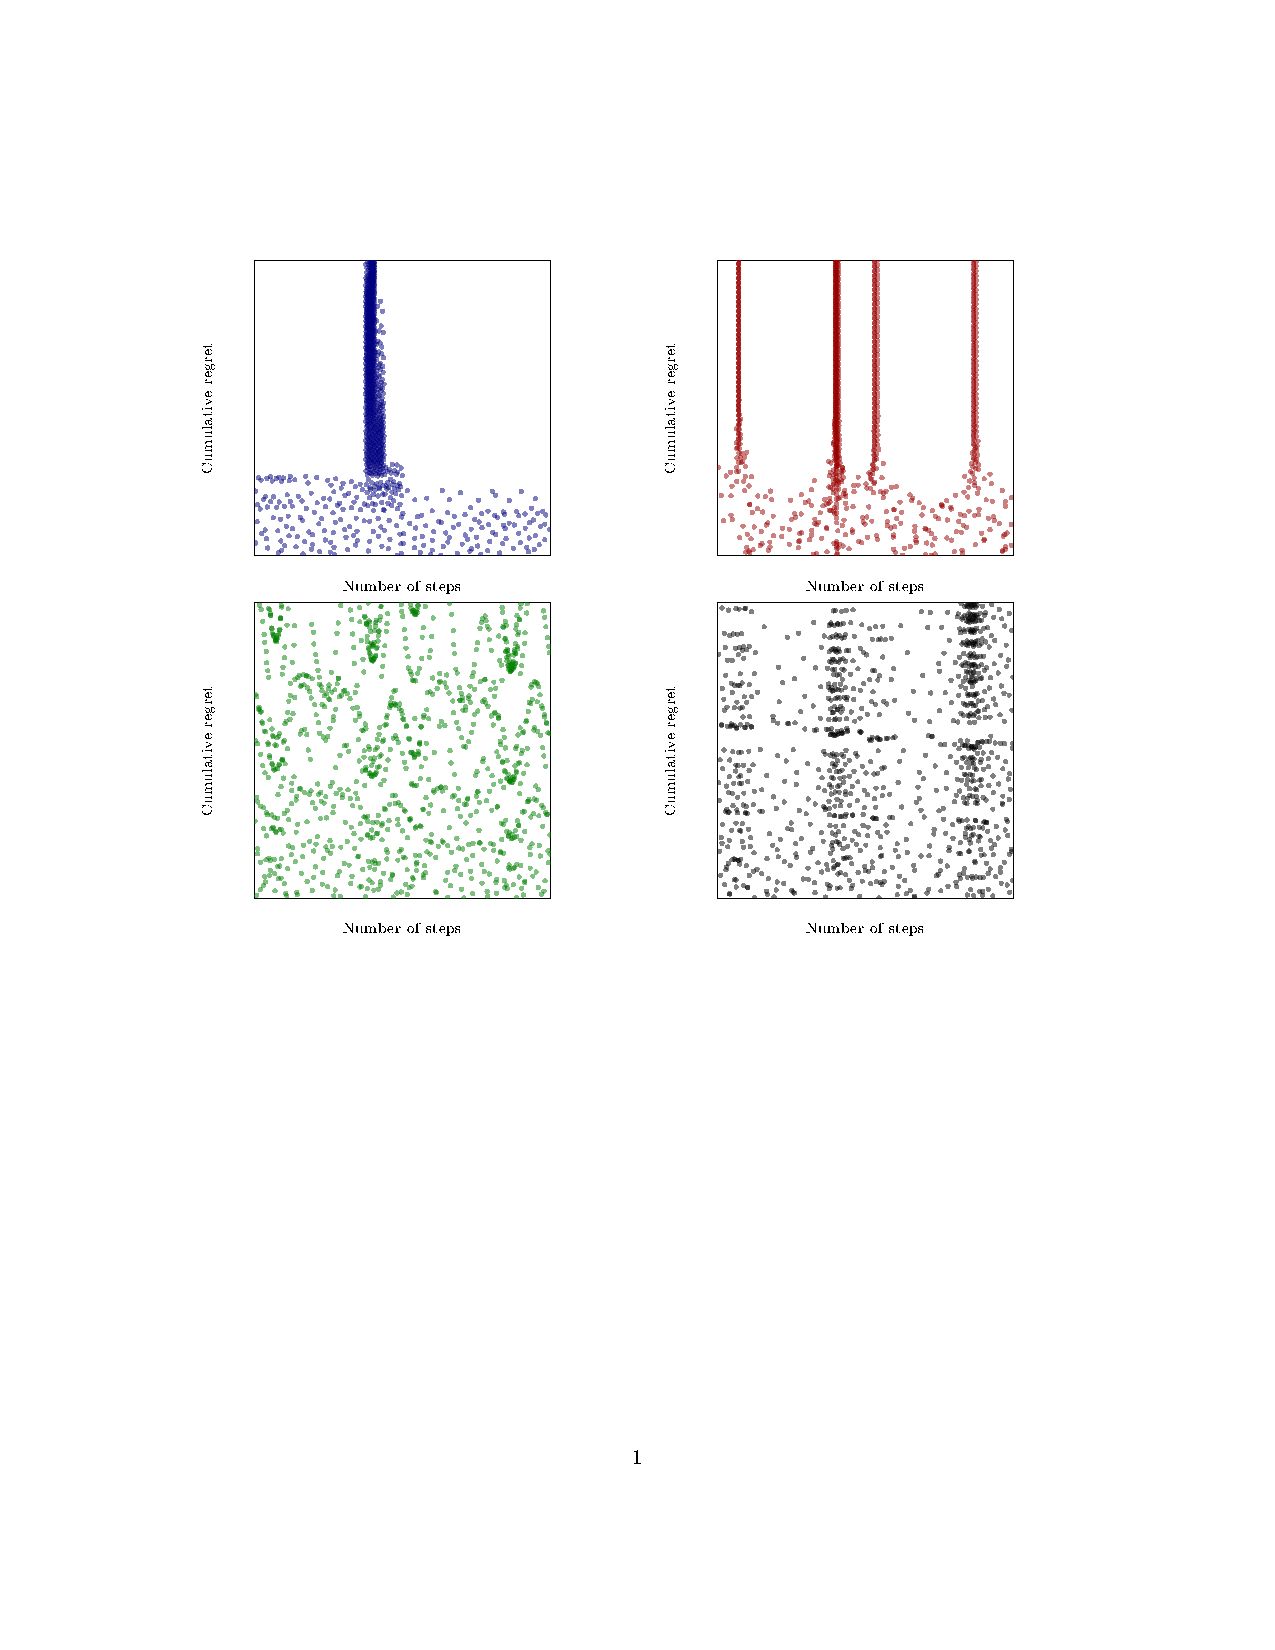
\includegraphics[trim = {0 6cm 0 4cm},clip,scale = 0.5]{marginal1000.pdf}
\vspace{-2.75cm}
  \caption{\label{fig:position1000}Points sampled by the algorithms for Sinprod with 1000 evaluations. From top left to bottom right : HOO, POO, HCT and StoSOO. For this function, $x^*\simeq 0.86$ and the second best point is roughly in $0.39$.}
\end{figure}
\end{frame}
%%%%%%%%%%%%%%%%%%%%%%%%%%% CUMULATIVE 1000 POINTS %%%%%%%%%%%%%%%%%%%%
\begin{frame}
\frametitle{Cumulative Regret}
%\hspace*{-2cm}
%\hfill
\vfill
\begin{figure}
	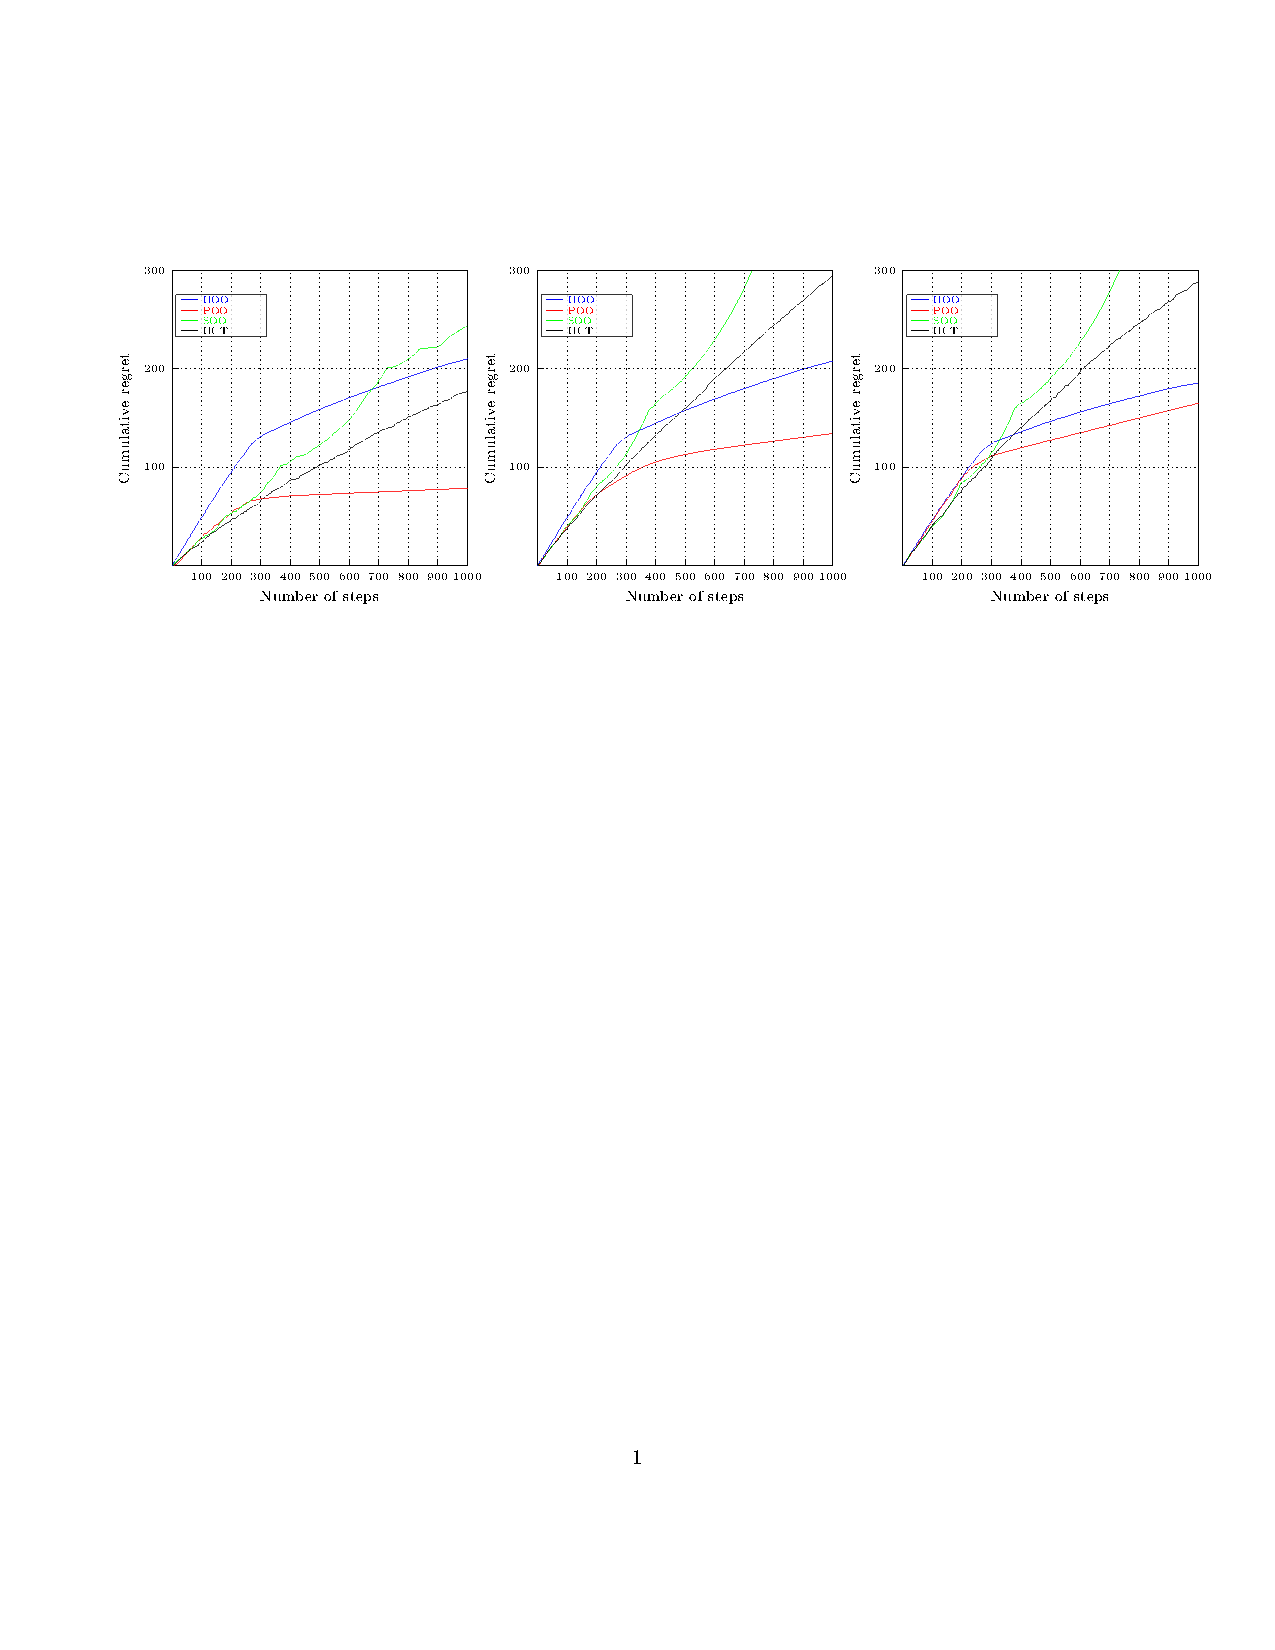
\includegraphics[trim={2cm 6cm 0 4cm},clip,scale = 0.65]{cumulative1000.pdf}
\vspace{-7.25cm}
\caption{\label{fig:cumulative1000}The cumulative regret of the 5 algorithms on the three difficult functions, with 1000 evaluations. From left to right : Grill function, Garland function, Sinprod function.}
\end{figure}
\end{frame}

%%%%%%%%%%%%%%%%%%%%%%%%%%% NOISE = 0.1 %%%%%%%%%%%%%%%%%%%%
\begin{frame}
\frametitle{Noised best estimator}
\begin{figure}
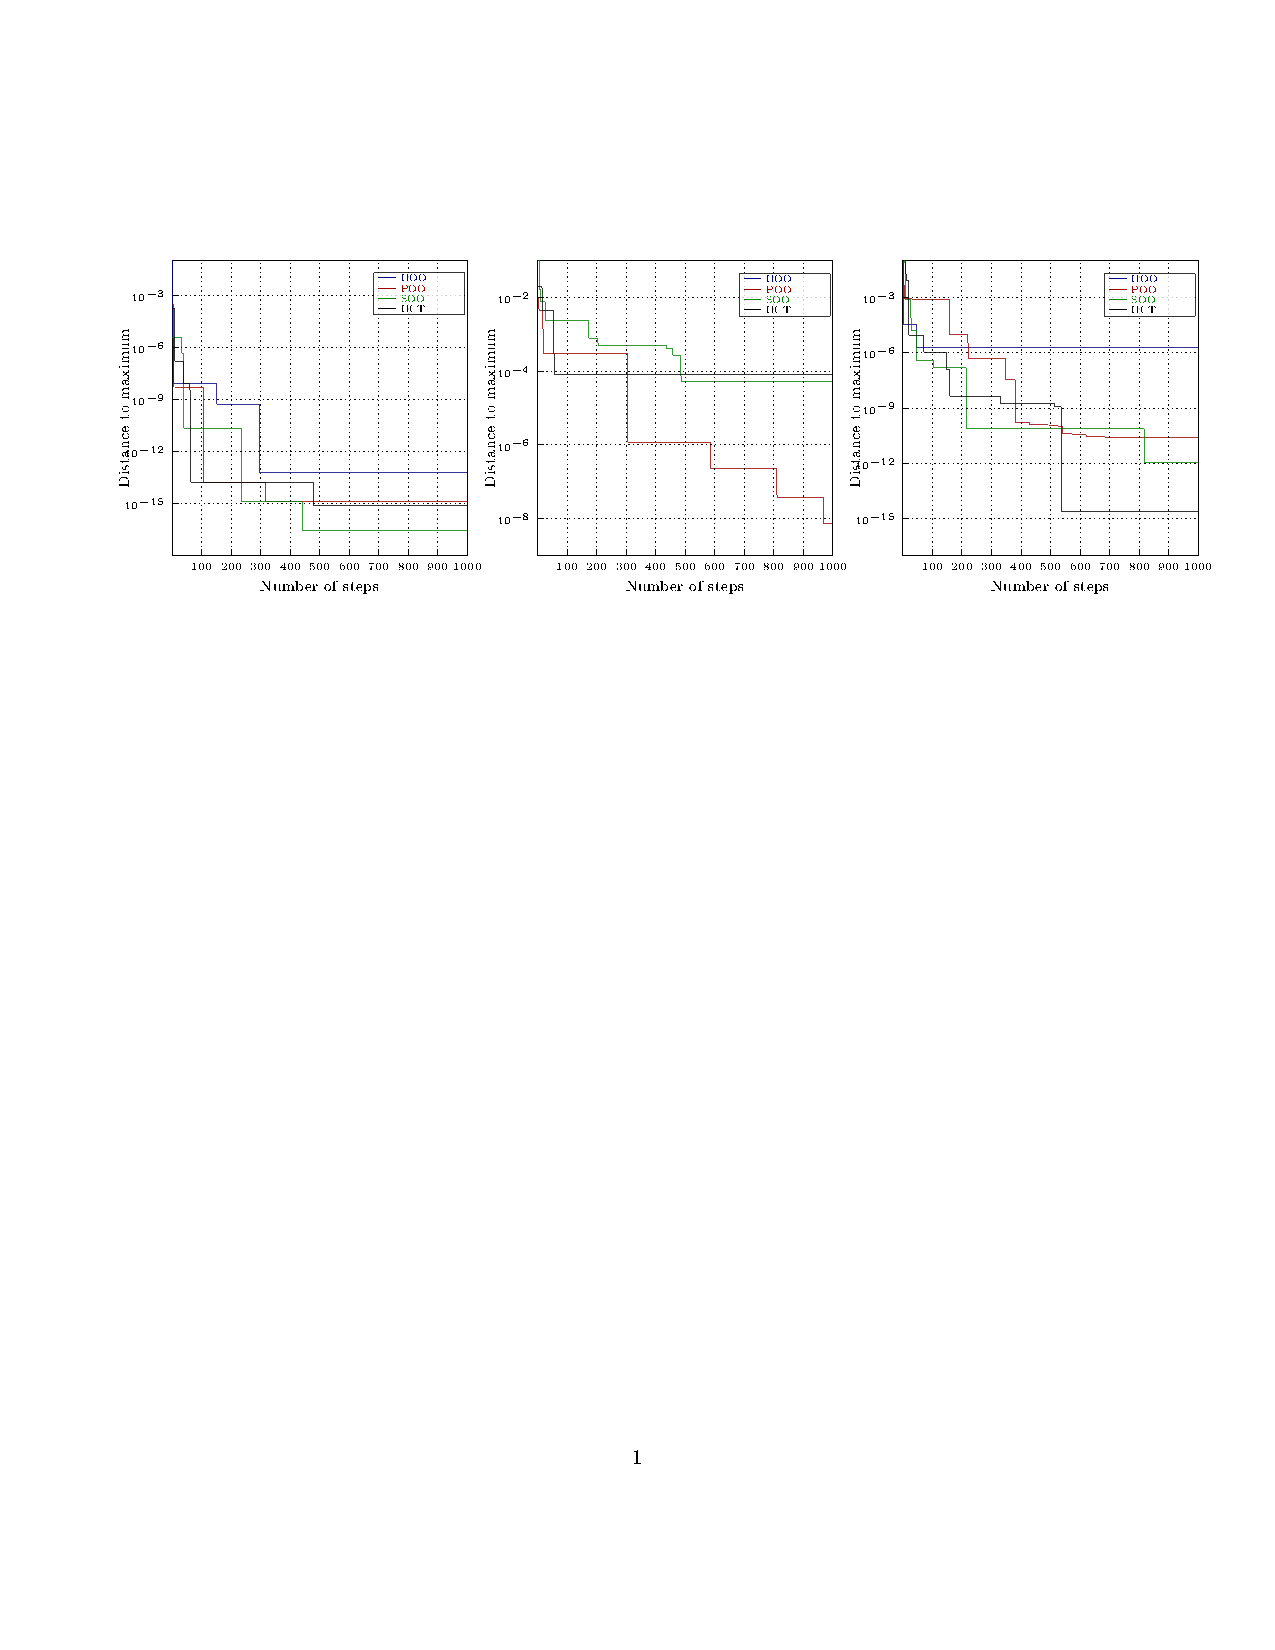
\includegraphics[trim={2cm 6cm 1cm 4cm},clip,scale = 0.65]{best1000_01.pdf}\\
\vspace*{-8cm}
 \caption{\label{fig:noise01}Best current regret under noisy estimation sampled from $\mathcal{N}(0,0.1)$ . From left to right : Grill function, Garland function, Sinprod function.}
\end{figure}
\end{frame}
\begin{frame}
\begin{figure}
\frametitle{Noised best estimator}
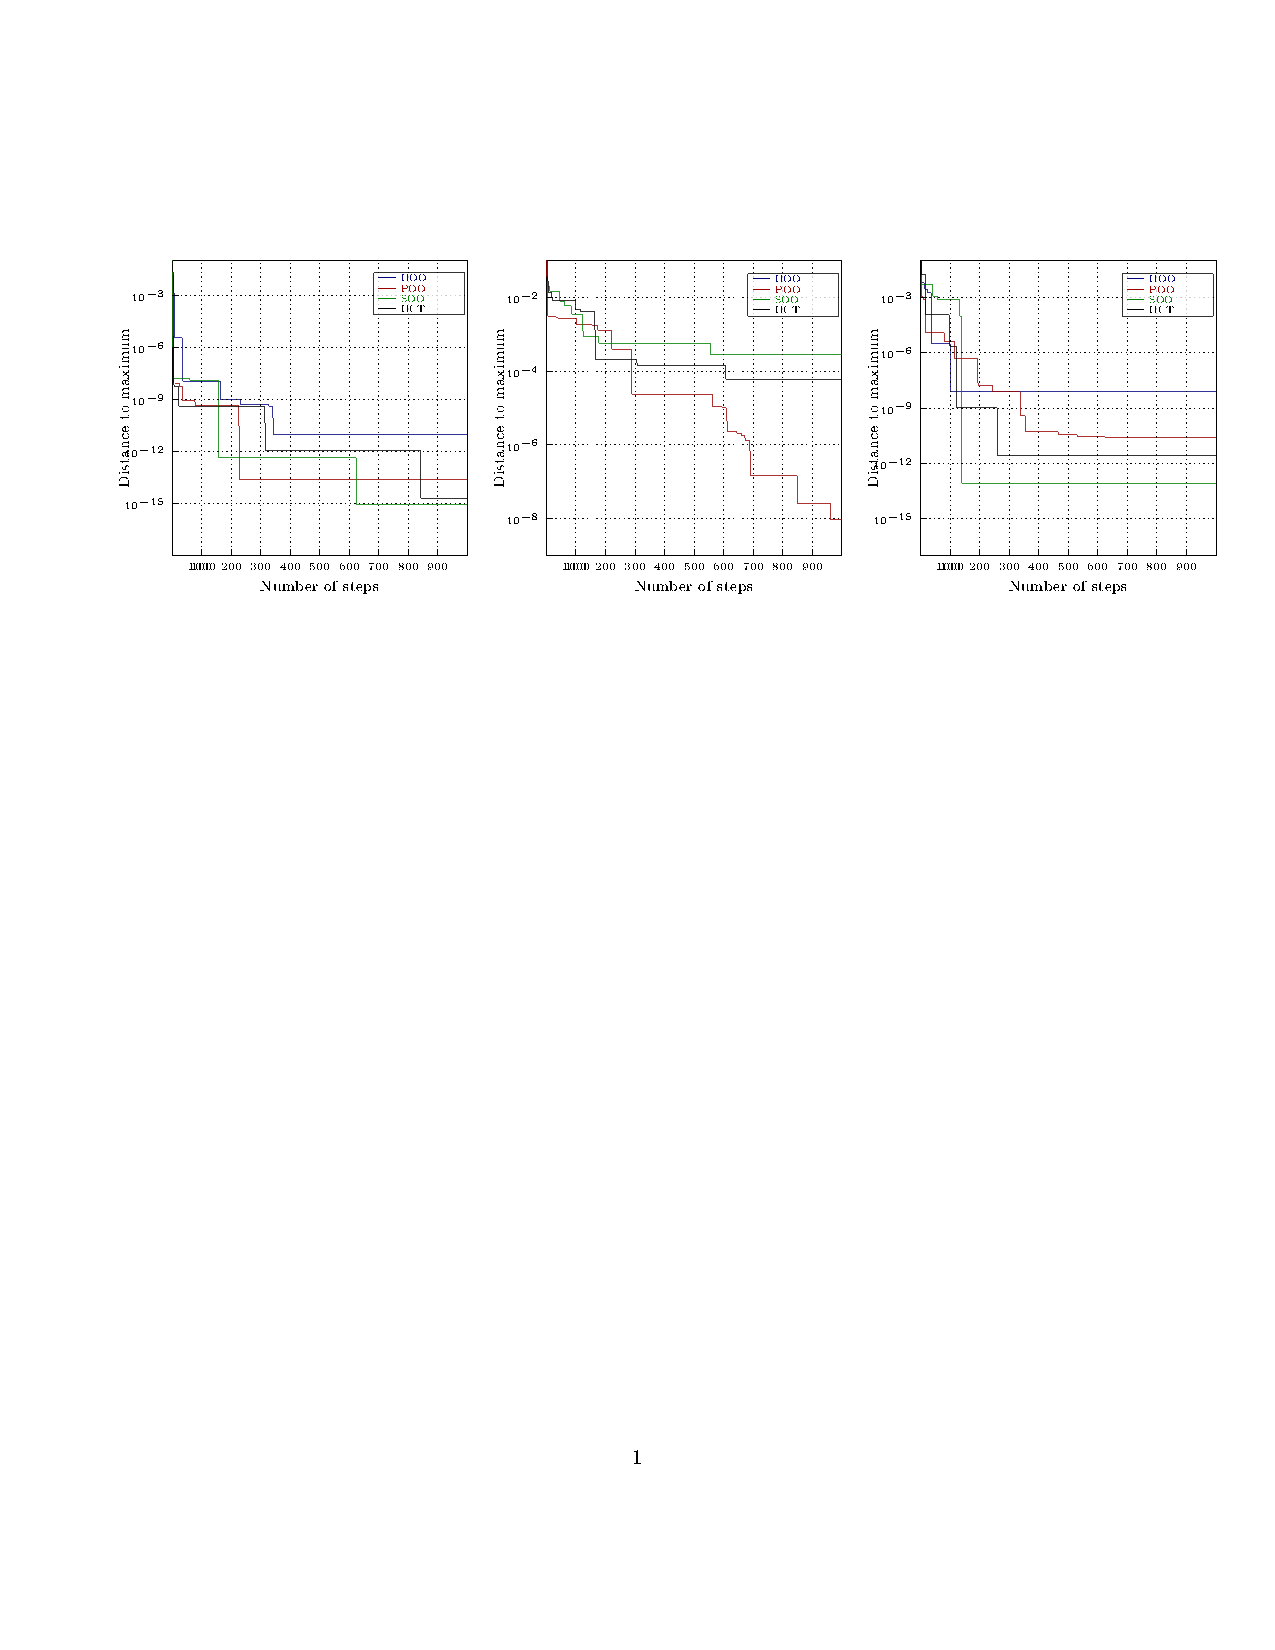
\includegraphics[trim={2cm 6cm 1cm 4cm},clip,scale = 0.65]{best1000_1.pdf}
\vspace*{-8cm}
 \caption{\label{fig:noise1}Best current regret under noisy estimation sampled from $\mathcal{N}(0,1)$. From left to right : Grill function, Garland function, Sinprod function.}
\end{figure}
\end{frame}

%%%%%%%%%%%%%%%%%%%%%%%%%%% ATB %%%%%%%%%%%%%%%%%%%%
\begin{frame}
\frametitle{ATB results}
\vspace{1cm}
\begin{figure}
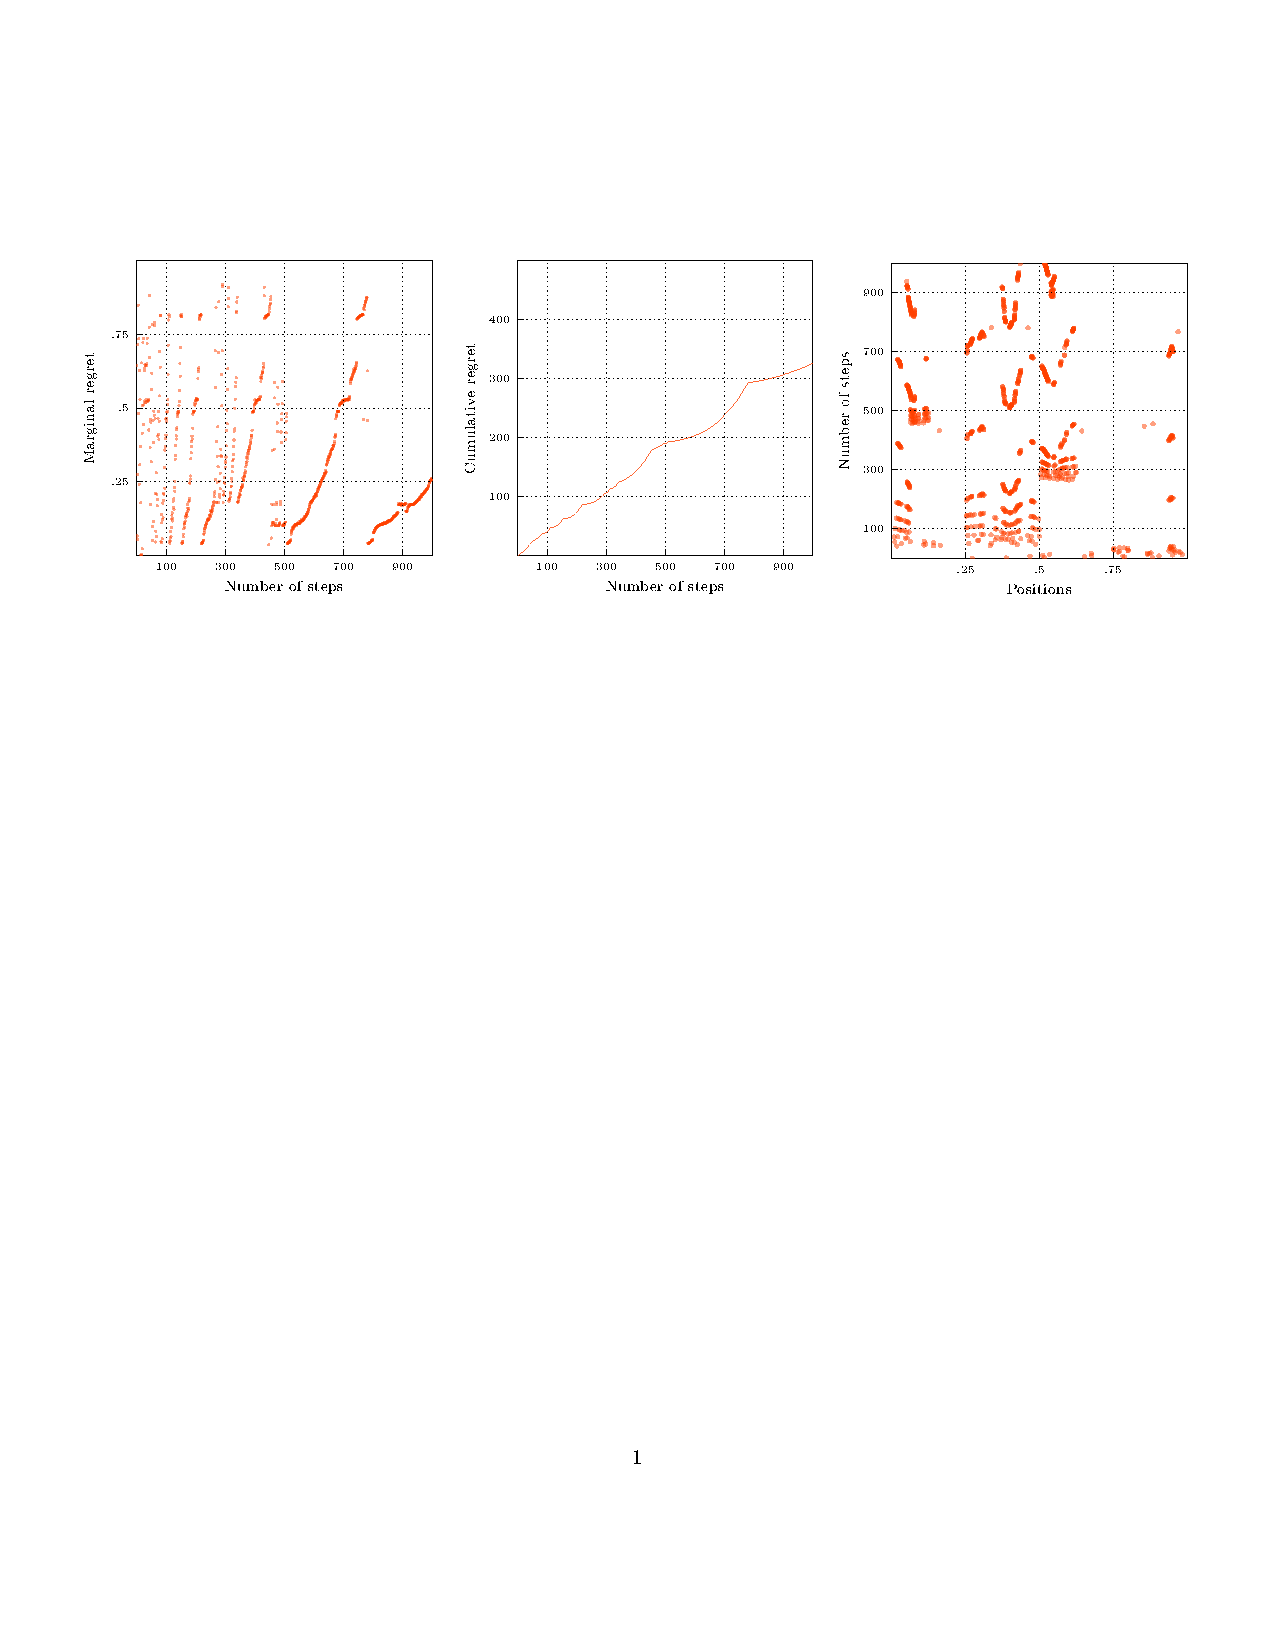
\includegraphics[trim={1cm 6cm 1cm 4cm},clip,scale = 0.64]{ATB.pdf}
\vspace*{-7cm}
\caption{\label{fig:atb}From the left to the right: simple and cumulative regrets and sampled points for ATB algorithm on Sinprod optimization.}
\end{figure}
\end{frame}
%%%% BIBILIOGRAPHY %%%%
\begin{frame}
	\small{
\bibliographystyle{plain}
\bibliography{Biblio}{}
\nocite{*}
}
\label{lastpage}
\end{frame}


\end{document}
